\documentclass{beamer}

% \usepackage[T1]{fontenc}
\usepackage{tcolorbox}
\usepackage{graphicx}
\usepackage{lmodern}
\usepackage{tabularx}
\usepackage{tikz}
\usepackage{blindtext}
\usepackage{svg}
\usepackage{booktabs}
\usepackage[style = ieee]{biblatex}
\usepackage{blindtext}
\usepackage{setspace}
\usepackage{minted}
\usepackage{nicematrix}
\usepackage{framed}
\usepackage{colortbl}
\usepackage{multirow}
\usepackage{multicol}
\usepackage{subfiles}

\usetikzlibrary{calc}
\usetikzlibrary{intersections,decorations.markings}

\usetikzlibrary{positioning}
\usetikzlibrary{ext.topaths.arcthrough}

\usepackage{subtikzpicture}

\usemintedstyle{dracula}

\renewcommand{\tabularxcolumn}[1]{m{#1}}

\makeatletter
\tikzset{
  use path for main/.code={%
    \tikz@addmode{%
      \expandafter\pgfsyssoftpath@setcurrentpath\csname tikz@intersect@path@name@#1\endcsname
    }%
  },
  use path for actions/.code={%
    \expandafter\def\expandafter\tikz@preactions\expandafter{\tikz@preactions\expandafter\let\expandafter\tikz@actions@path\csname tikz@intersect@path@name@#1\endcsname}%
  },
  use path/.style={%
    use path for main=#1,
    use path for actions=#1,
  }
}

\definecolor{forestbg}      {RGB} {31, 30, 24}

\def\leafColorPrimaryName{Sage}
\def\leafColorPrimaryRGB{138, 184, 114}
\def\leafColorPrimaryHex{\#8AB872}
\definecolor{leafColorPrimary} {RGB} {\leafColorPrimaryRGB}
%%
\def\leafColorSecondaryName{Cactus Spike}
\def\leafColorSecondaryRGB{204, 224, 153}
\def\leafColorSecondaryHex{\#CCE099}
\definecolor{leafColorSecondary} {RGB} {\leafColorSecondaryRGB}

\definecolor{colorBlue}   {HTML} {33539E}
\definecolor{colorSky}    {HTML} {7FACD6}
\definecolor{colorViolet} {HTML} {BFB8DA}
\definecolor{colorPink}   {HTML} {E8B7D4}
\definecolor{colorMaroon} {HTML} {A5678E}

\definecolor{colorRampart} {HTML} {BDB7B7}
\definecolor{colorCaramel} {HTML} {B89B93}
\definecolor{colorCortex} {HTML} {A59691}
\definecolor{colorDove} {HTML} {B6AFA5}
\definecolor{colorCathedral} {HTML} {ABA7A6}
\definecolor{colorWind} {HTML} {CAC4C4}

\definecolor{colorRed} {HTML} {E44E54}
\colorlet{colorLightRed}{colorRed!50!white}
% \definecolor{colorLightRed} {HTML} {F46367}
\definecolor{colorVeryLightRed} {HTML} {D1AE97}
\definecolor{colorDarkRed} {HTML} {581319}
\definecolor{colorDarkGreen} {HTML} {2E4330}
\definecolor{colorLightGreen} {HTML} {C0D2A3}

\definecolor{colorLightBrown} {HTML} {A8867B}
\definecolor{colorLightSageGreen} {HTML} {9EC2AD}

\definecolor{colorBrown} {HTML} {9F774E}

\definecolor{colorTest} {HTML} {133330}

\newcommand\tableBox[2] {
    \begin{tcolorbox}[
            coltitle = leafColorPrimary,
            colbacktitle = leafColorSecondary,
            colback = leafColorSecondary,
            colframe = leafColorSecondary,
            title=#1,
            fonttitle=\bfseries,
            detach title,
        ]
        \begin{minipage}[t]{0.1\textwidth}
            \begin{flushleft}
                \tcbtitle
            \end{flushleft}
        \end{minipage}
        \begin{minipage}[t]{0.9\textwidth}
            #2
        \end{minipage}
    \end{tcolorbox}
}

\newcommand\tikzframetitleleft[2] {
    \draw (current page.north west) ++(0.75cm, -0.75cm) coordinate (frametitle) ;
    \node [anchor = north west] (frametitle) at (frametitle) {
        \begin{minipage} {9cm}
            \bfseries
            \setstretch{0.75}
            \huge
            {\Large #1} \\ #2
        \end{minipage}
    }
    ;
}

\newcommand\tikzframetitlelongleft[2] {
    \draw (current page.north west) ++(0.75cm, -0.75cm) coordinate (frametitle) ;
    \node [anchor = north west] (frametitle) at (frametitle) {
        \begin{minipage} {10cm}
            \bfseries
            \setstretch{0.75}
            \huge
            {\Large #1} \\ #2
        \end{minipage}
    }
    ;
}

\newcommand\tikzframetitleright[2] {
    \draw (current page.north east) ++(-0.75cm, -0.75cm) coordinate (frametitle) ;
    \node [anchor = north east] (frametitle) at (frametitle) {
        \begin{minipage} {9cm}
            \bfseries
            \raggedleft
            \setstretch{0.75}
            \huge
            {\Large #1} \\ #2
        \end{minipage}
    }
    ;
}

\newcommand\tikzframetitlelongright[2] {
    \draw (current page.north east) ++(-0.75cm, -0.75cm) coordinate (frametitle) ;
    \node [anchor = north east] (frametitle) at (frametitle) {
        \begin{minipage} {11cm}
            \bfseries
            \raggedleft
            \setstretch{0.75}
            \huge
            {\Large #1} \\ #2
        \end{minipage}
    }
    ;
}
\colorlet{fgcol}{colorDarkGreen}

\def\markMainInnerRadius{0.175cm}
\def\markMainOuterRadius{0.3cm}
\def\markSubRadius{0.075cm}
\def\markCornerRadius{0.1cm}


% \usepackage{minted}

\usepackage[size=custom,width=16,height=9,scale=0.4]{beamerposter}
% \usepackage[size=custom, width=12.8, height=9.6, scale=0.4]{beamerposter}

\usepackage[T1]{fontenc}
\usepackage{tcolorbox}
\usepackage{graphicx}
\usepackage{lmodern}
\usepackage{tabularx}
\usepackage{tikz}
\usepackage{blindtext}
\usepackage{svg}
\usepackage{fontspec}
\usepackage{booktabs}
\usepackage[style = ieee]{biblatex}
\usepackage{blindtext}
\usepackage{setspace}
\usepackage{minted}
\usepackage{nicematrix}

\usetikzlibrary{calc}
\usetikzlibrary{intersections,decorations.markings}

\usemintedstyle{dracula}

\makeatletter
\tikzset{
  use path for main/.code={%
    \tikz@addmode{%
      \expandafter\pgfsyssoftpath@setcurrentpath\csname tikz@intersect@path@name@#1\endcsname
    }%
  },
  use path for actions/.code={%
    \expandafter\def\expandafter\tikz@preactions\expandafter{\tikz@preactions\expandafter\let\expandafter\tikz@actions@path\csname tikz@intersect@path@name@#1\endcsname}%
  },
  use path/.style={%
    use path for main=#1,
    use path for actions=#1,
  }
}
\setsansfont{Garamond.ttf}

% \usefonttheme{serif}
% \usepackage{beamercolorthemedracula}

% \addbibresource{abstract.bib} %Import the bibliography file

\usetheme{metropolis}

\definecolor{forestbg}      {RGB} {31, 30, 24}

\title{TinyML in Agriculture Sector}

\subtitle{Awakening of Minds in Low Power Edge Devices}

\date{\today}

\author{
    Daniel V Mathew
}

\institute{Rajiv Gandhi Institute of Technology, Kottayam}

\def\supervisor{
    Prof. Sujithamol S
}

\def\leafColorPrimaryName{Sage}
\def\leafColorPrimaryRGB{138, 184, 114}
\def\leafColorPrimaryHex{\#8AB872}
\definecolor{leafColorPrimary} {RGB} {\leafColorPrimaryRGB}
%%
\def\leafColorSecondaryName{Cactus Spike}
\def\leafColorSecondaryRGB{204, 224, 153}
\def\leafColorSecondaryHex{\#CCE099}
\definecolor{leafColorSecondary} {RGB} {\leafColorSecondaryRGB}

\definecolor{colorBlue}   {HTML} {33539E}
\definecolor{colorSky}    {HTML} {7FACD6}
\definecolor{colorViolet} {HTML} {BFB8DA}
\definecolor{colorPink}   {HTML} {E8B7D4}
\definecolor{colorMaroon} {HTML} {A5678E}

\definecolor{colorRampart} {HTML} {BDB7B7}
\definecolor{colorCaramel} {HTML} {B89B93}
\definecolor{colorCortex} {HTML} {A59691}
\definecolor{colorDove} {HTML} {B6AFA5}
\definecolor{colorCathedral} {HTML} {ABA7A6}
\definecolor{colorWind} {HTML} {CAC4C4}

\definecolor{colorRed} {HTML} {E44E54}
\definecolor{colorLightRed} {HTML} {F46367}
\definecolor{colorVeryLightRed} {HTML} {D1AE97}
\definecolor{colorDarkRed} {HTML} {581319}
\definecolor{colorDarkGreen} {HTML} {2E4330}
\definecolor{colorLightGreen} {HTML} {C0D2A3}

\definecolor{colorLightBrown} {HTML} {A8867B}
\definecolor{colorDarkBrown} {HTML} {9EC2AD}

\definecolor{colorBrown} {HTML} {9F774E}

\definecolor{colorTest} {HTML} {133330}

\renewcommand\alert[1] {%
    {\color{colorRed}#1}%
}

\newcommand\tableBox[2] {
    \begin{tcolorbox}[
            coltitle = leafColorPrimary,
            colbacktitle = leafColorSecondary,
            colback = leafColorSecondary,
            colframe = leafColorSecondary,
            title=#1,
            fonttitle=\bfseries,
            detach title,
        ]
        \begin{minipage}[t]{0.1\textwidth}
            \begin{flushleft}
                \tcbtitle
            \end{flushleft}
        \end{minipage}
        \begin{minipage}[t]{0.9\textwidth}
            #2
        \end{minipage}
    \end{tcolorbox}
}

% \setbeamertemplate{background} {
%     \begin{tikzpicture} [remember picture, overlay]
%         \filldraw [
%             colorWind,
%         ]
%         (current page.north west) rectangle (current page.south east)
%         ;
%     \end{tikzpicture}
% }

% \setbeamertemplate{frametitle}{
%     \begin{tikzpicture} [remember picture, overlay]
%         \node (title) at (current page.north west) [
%             black, anchor = north west
%         ] {\strut\insertframetitle\strut};
%         \draw[
%             black,
%             very thick,
%             line cap = round,
%         ]
%         (title.east) -- (title.east -| current page.east)
%         ;
%     \end{tikzpicture}%
% }

\setbeamercolor{frametitle}{%
  fg=white,
  bg=colorMaroon
}

\newcommand\tikzframetitleleft[2] {
    \draw (current page.north west) ++(0.75cm, -0.75cm) coordinate (frametitle) ;
    \node [anchor = north west] (frametitle) at (frametitle) {
        \begin{minipage} {8cm}
            \setstretch{0.75}
            \huge
            {\Large #1} \\ #2
        \end{minipage}
    }
    ;
}

\newcommand\tikzframetitleright[2] {
    \draw (current page.north east) ++(-0.75cm, -0.75cm) coordinate (frametitle) ;
    \node [anchor = north east] (frametitle) at (frametitle) {
        \begin{minipage} {8cm}
            \raggedleft
            \setstretch{0.75}
            \huge
            {\Large #1} \\ #2
        \end{minipage}
    }
    ;
}

\colorlet{fgcol}{colorDarkGreen}

\def\markMainInnerRadius{0.175cm}
\def\markMainOuterRadius{0.3cm}
\def\markSubRadius{0.075cm}
\def\markCornerRadius{0.1cm}

\begin{document}

\maketitle

% \begin{frame} {Introduction}
%     \begin{tikzpicture}
%
%         \draw (0, 0) coordinate (tmp);
%         \foreach \x in {
%             colorDarkGreen,
%             colorRed,
%             colorBlue,
%             colorSky,
%             colorViolet,
%             colorPink,
%             colorMaroon,
%             %%
%             colorRampart,
%             colorCaramel,
%             colorCortex,
%             colorDove,
%             colorCathedral%
%         } {
%             \filldraw [ \x ] (tmp) circle (1cm) (tmp) ++(1.5, 0) coordinate (tmp);
%         }
%
%     \end{tikzpicture}
% \end{frame}

%% Making Sense of Data
\begin{frame} {}

    \begin{tikzpicture} [
            remember picture,
            overlay,
        ]

        \draw (0, 0)
        coordinate (origin)
        (current page.east) ++(1, 0) coordinate (edge)
        ;

        \begin{scope}
            %% Humidity
            \draw []
            (current page.south) ++(1.0cm, 2.5cm) coordinate (humidityMarkCenter)
            ;
            \path [name path = markHumeHandle, rounded corners = \markCornerRadius]
            (humidityMarkCenter) ++(135:\markMainOuterRadius) coordinate (humidityMarkFirst)
            (humidityMarkCenter) ++(135:(0.75cm + \markMainOuterRadius) coordinate (humidityMarkSecond)
            (humidityMarkSecond) ++(-1, 0) coordinate (humidityMarkThird)
            (humidityMarkFirst) -- (humidityMarkSecond) -- (humidityMarkThird)
            ;
            \draw [use path = markHumeHandle, very thick] ;
            ;
            \filldraw [fgcol]
            (humidityMarkThird) circle (\markSubRadius)
            ;
            \draw [fgcol]
            (humidityMarkThird) node [left = 6pt] {
                Humidity Data
            }
            ;

            %% Temperature
            \draw []
            (current page.south) ++(5.0cm, 6.55cm) coordinate (temperatureMarkCenter)
            ;
            \path [name path = markTempHandle, rounded corners = \markCornerRadius]
            (temperatureMarkCenter) ++(135:\markMainOuterRadius) coordinate (temperatureMarkFirst)
            (temperatureMarkCenter) ++(135:(0.75cm + \markMainOuterRadius) coordinate (temperatureMarkSecond)
            (temperatureMarkSecond) ++(-1, 0) coordinate (temperatureMarkThird)
            (temperatureMarkFirst) -- (temperatureMarkSecond) -- (temperatureMarkThird)
            ;
            \draw [use path = markTempHandle, very thick] ;
            ;
            \filldraw [fgcol]
            (temperatureMarkThird) circle (\markSubRadius)
            ;
            \draw [fgcol]
            (temperatureMarkThird) node [left = 6pt] {
                Temperature Data
            }
            ;

            \clip [rotate = 45, rounded corners = 0.7cm]
            (edge) ++(-10, -15) rectangle ++(20, 20)
            ;

            \begin{scope}
                \node [anchor = east] (img) at (edge) {
                    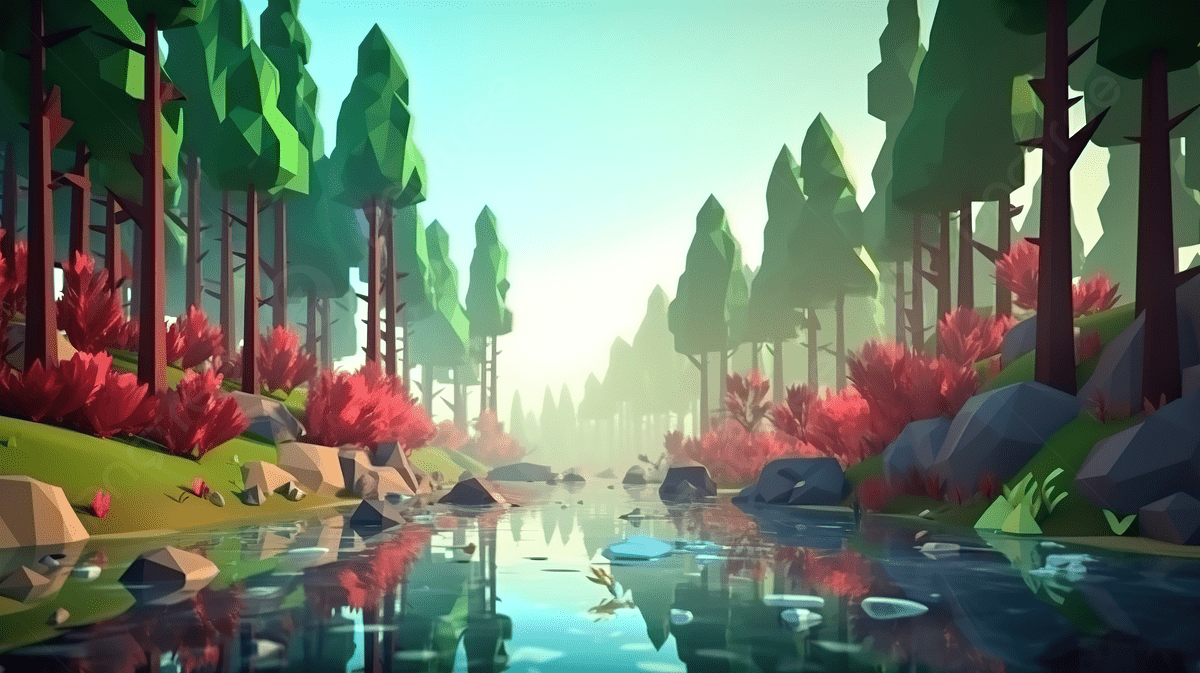
\includegraphics[height = \paperheight]{low.jpg}
                }
                ;

                %% Humidity
                \filldraw [white!90!fgcol]
                (humidityMarkCenter) circle (\markMainInnerRadius)
                ;
                \draw [white!90!fgcol, very thick]
                (humidityMarkCenter) circle (\markMainOuterRadius)
                ;
                \draw [use path = markHumeHandle, white!90!fgcol, very thick] ;

                %% Temperature
                \filldraw [white!90!fgcol]
                (temperatureMarkCenter) circle (\markMainInnerRadius)
                ;
                \draw [white!90!fgcol, very thick]
                (temperatureMarkCenter) circle (\markMainOuterRadius)
                ;
                \draw [use path = markTempHandle, white!90!fgcol, very thick] ;

            \end{scope}
        \end{scope}

        \tikzframetitleleft{Making} {Sense of Data}

        \draw (frametitle.south west) ++(0, -0.5cm) coordinate (content) ;
        \node [anchor = north west]  (content) at (content) {
            \begin{minipage} {6cm}
                \begin{itemize}[]
                    \item Say something.
                    \item Interesting.
                \end{itemize}
            \end{minipage}
        }
        ;

        \draw (0, 0)
        coordinate (origin)
        (current page.west) coordinate (edge)
        ;
        \begin{scope} [transform canvas = {yshift = -2.2cm, xshift = 0.5cm}]
            \draw []
            (edge) ++(2cm, -0.5cm) coordinate (pixelMarkCenter)
            ;
            \path [name path = markHandle, rounded corners = \markCornerRadius]
            (pixelMarkCenter) ++(-45:\markMainOuterRadius) coordinate (pixelMarkFirst)
            (pixelMarkCenter) ++(-45:(1cm + \markMainOuterRadius) coordinate (pixelMarkSecond)
            (pixelMarkSecond) ++(1, 0) coordinate (pixelMarkThird)
            (pixelMarkFirst) -- (pixelMarkSecond) -- (pixelMarkThird)
            ;
            \draw [use path = markHandle, very thick] ;
            \filldraw [fgcol]
            (pixelMarkThird) circle (\markSubRadius)
            ;
            \draw [fgcol]
            (pixelMarkThird) node [right = 6pt] {
                Pixel Data
            }
            ;
            \clip [rotate = -45, rounded corners = 0.7cm]
            (edge) rectangle ++(2.5, 2.5)
            ;
            \begin{scope}
                \node [anchor = west] (pixel) at (edge) {
                    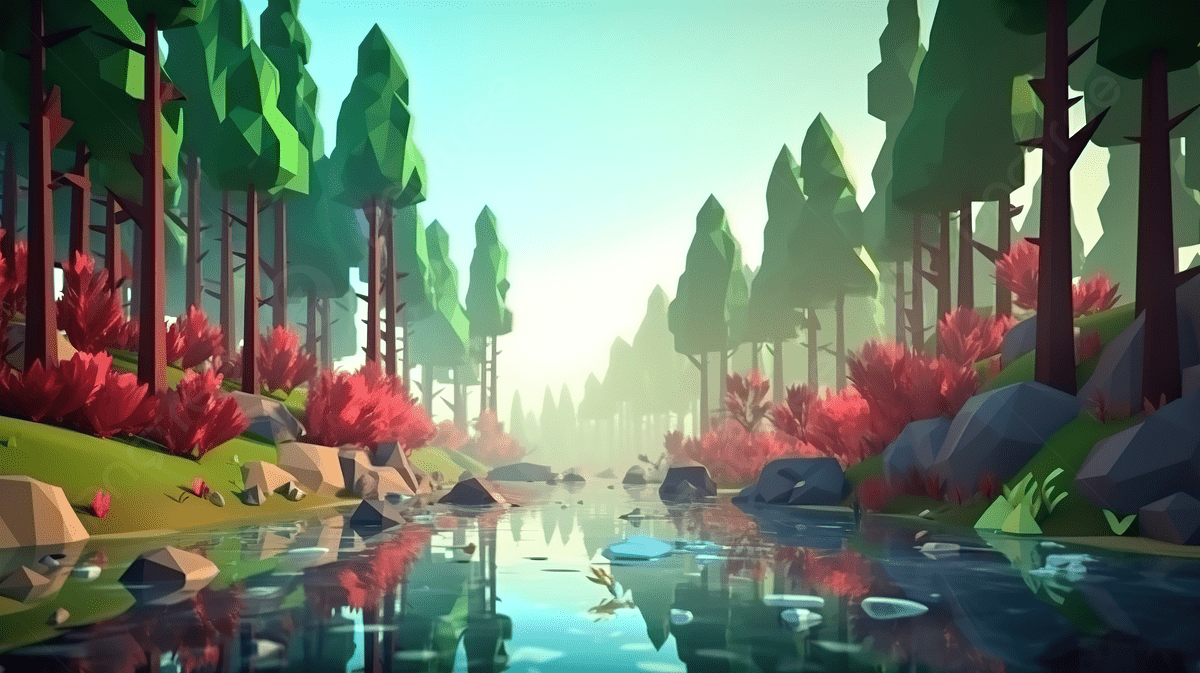
\includegraphics[height = \paperheight]{low.jpg}
                }
                ;
                \draw [thin, step = 0.1, white, opacity = 0.40]
                (edge) ++(-1, -2) grid ++(5, 5)
                ;
                \filldraw [white!90!fgcol]
                (pixelMarkCenter) circle (\markMainInnerRadius)
                ;

                \draw [white!90!fgcol, very thick]
                (pixelMarkCenter) circle (\markMainOuterRadius)
                ;
                \draw [use path = markHandle, white!90!fgcol, very thick] ;
            \end{scope}
        \end{scope}

    \end{tikzpicture}

\end{frame}

%% Learning to Ask the Right Questions
\begin{frame} {}

    \begin{tikzpicture} [
            remember picture,
            overlay,
        ]
        \tikzframetitleleft{Asking}{The Right Questions}

        \draw (frametitle.south west) ++(0, -0.5cm) coordinate (content) ;
        \node [anchor = north west]  (content) at (content) {
            \begin{minipage} {0.45\paperwidth}
                In order to make sense of the data, we need to ask the right questions about the data.
                The sequence of these questions is known as an \alert{Algorithm}.
            \end{minipage}
        }
        ;

        \filldraw [colorTest]
        (current page.north east) ++(-7,0) coordinate (workFlowTop)
        (workFlowTop) rectangle (current page.south east)
        ;

        \draw (workFlowTop) ++(0, -0.2) coordinate (tmp);
        \foreach \x in {1, 2, 3, 4} {
            \draw [very thick, white, rounded corners = 0.2cm, line cap = round]
            (tmp) ++(0, -1) -- ++(3.5, -0.8) -- ++(3.5, 0.8)
            (tmp) ++(0, -0.25\paperheight) coordinate (tmp)
            ;
        }

        \draw ($(workFlowTop)!0.5!(current page.north east)$) ++(0, -0.8) coordinate (tmp);
        \foreach \x in {
            Finding a Problem,
            Selecting an Algorithm,
            Implementing the Algorithm,
            Solving the Problem%
        } {
            \draw [ultra thick, white, rounded corners = 0.2cm]
            (tmp)
            node [anchor = center] {
                \begin{minipage} {7cm}
                    \centering
                    \x
                \end{minipage}
            }
            % (tmp) ++(0, -1) -- ++(3.5, -1.25) -- ++(3.5, 1.25)
            (tmp) ++(0, -0.25\paperheight) coordinate (tmp)
            ;
        }

        %% Methodology

        \begin{scope}
            \draw
            (current page.center) ++(1.75cm, 0) coordinate (workFlowMarkCenter)
            % (current page.center) ++(1.6cm, 0.2cm) coordinate (workFlowMarkCenter)
            ;
            \path [name path = markWorkHandle, rounded corners = \markCornerRadius]
            (workFlowMarkCenter) ++(-180:\markMainOuterRadius) coordinate (workFlowMarkFirst)
            (workFlowMarkFirst) ++(-1, 0) coordinate (workFlowMarkSecond)
            (workFlowMarkSecond) ++(-135:0.75cm) coordinate (workFlowMarkThird)
            (workFlowMarkFirst) -- (workFlowMarkSecond) -- (workFlowMarkThird)
            ;
            \draw [use path = markWorkHandle, very thick] ;
            \filldraw [fgcol]
            (workFlowMarkThird) circle (\markSubRadius)
            ;
            \draw [fgcol]
            (workFlowMarkThird) node (workFlowMark) [left = 6pt] {
                Typical Way of Solving a Problem
            }
            ;
            \clip (workFlowTop) rectangle (current page.south east);
            \begin{scope}
                \filldraw [white!90!fgcol]
                (workFlowMarkCenter) circle (\markMainInnerRadius)
                ;
                \draw [white!90!fgcol, very thick]
                (workFlowMarkCenter) circle (\markMainOuterRadius)
                ;
                \draw [white!90!fgcol, use path = markWorkHandle, very thick] ;
            \end{scope}
        \end{scope}

        \draw (content.south west |- workFlowMark.south west) ++(0, -0.5cm) coordinate (content) ;
        \node [anchor = north west]  (content) at (content) {
            \begin{minipage} {0.45\paperwidth}
                But what if the sheer number of questions one must ask to get to the right answer gets
                so overwhelming?
            \end{minipage}
        }
        ;

        \draw (content.south west) ++(0, -0.5cm) coordinate (content) ;
        \node [anchor = north west]  (content) at (content) {
            \begin{minipage} {0.45\paperwidth}
                But before that...
            \end{minipage}
        }
        ;

    \end{tikzpicture}

\end{frame}

%% Ways of Asking Questions
\begin{frame}[fragile] {}

    \begin{tikzpicture} [
            remember picture,
            overlay
        ]
        \tikzframetitleright {Ways of} {Asking Questions}

        \begin{scope} [transform canvas = {xshift = 0.2cm}]
            \begin{scope}
                \draw
                (current page.north) ++(-0.75, -0.75) coordinate (ifelseMarkCenter)
                ;
                \path [name path = ifelseHandle, rounded corners = \markCornerRadius]
                (ifelseMarkCenter) ++(-45:\markMainOuterRadius) coordinate (ifelseMarkFirst)
                (ifelseMarkCenter) ++(-45:(2.85cm + \markMainOuterRadius) coordinate (ifelseMarkSecond)
                (ifelseMarkSecond) ++(1.4, 0) coordinate (ifelseMarkThird)
                (ifelseMarkFirst) -- (ifelseMarkSecond) -- (ifelseMarkThird)
                ;
                \draw [use path = ifelseHandle, very thick] ;
                \filldraw [
                    colorLightGreen,
                    rounded corners = 0.7cm,
                ]
                (current page.north west) ++(0, 0.1cm) ++(0,2) coordinate (tmpStart)
                (current page.center) ++(0, 0.1cm) coordinate (tmpEnd)
                (tmpStart) rectangle (tmpEnd)
                ;
                \filldraw [fgcol]
                (ifelseMarkThird) circle (\markSubRadius)
                ;
                \draw [fgcol]
                (ifelseMarkThird) node (ifelse) [right = 6pt] {
                    Using If-Else Statements
                }
                ;
                \clip [
                    rounded corners = 0.7cm,
                ]
                (current page.north west) ++(0, 0.1cm) ++(0,2) coordinate (tmpStart)
                (current page.center) ++(0, 0.1cm) coordinate (tmpEnd)
                (tmpStart) rectangle (tmpEnd)
                ;
                \begin{scope}
                    \filldraw [white!90!fgcol]
                    (ifelseMarkCenter) circle (\markMainInnerRadius)
                    ;
                    \draw [white!90!fgcol, very thick]
                    (ifelseMarkCenter) circle (\markMainOuterRadius)
                    ;
                    \draw [white!90!fgcol, use path = ifelseHandle, very thick] ;
                \end{scope}
            \end{scope}

            % \draw [thin, step = 0.1, white, opacity = 0.40]
            % (current page.north west) ++(-2,2) grid (current page.center)
            % ;

            \begin{scope}
                \draw
                (current page.south) ++(-0.75, 1.0) coordinate (matrixMarkCenter)
                ;
                \path [name path = matrixHandle, rounded corners = \markCornerRadius]
                (matrixMarkCenter) ++(45:\markMainOuterRadius) coordinate (matrixMarkFirst)
                (matrixMarkCenter) ++(45:(2.0cm + \markMainOuterRadius) coordinate (matrixMarkSecond)
                (matrixMarkSecond) ++(1.35, 0) coordinate (matrixMarkThird)
                (matrixMarkFirst) -- (matrixMarkSecond) -- (matrixMarkThird)
                ;
                \draw [use path = matrixHandle, very thick] ;
                \filldraw [
                    colorDarkBrown,
                    rounded corners = 0.7cm,
                ]
                (current page.south west) ++(0, -0.1cm) ++(0,-2) coordinate (tmpStart)
                (current page.center) ++(0, -0.1cm) coordinate (tmpEnd)
                (tmpStart) rectangle (tmpEnd)
                ;
                \filldraw [fgcol]
                (matrixMarkThird) circle (\markSubRadius)
                ;
                \draw [fgcol]
                (matrixMarkThird) node (matrix) [right = 6pt] {
                    Using Matrix Transformation
                }
                ;
                \clip [
                    rounded corners = 0.7cm,
                ]
                (current page.south west) ++(0, -0.1cm) ++(0,-2) coordinate (tmpStart)
                (current page.center) ++(0, -0.1cm) coordinate (tmpEnd)
                (tmpStart) rectangle (tmpEnd)
                ;
                \begin{scope}
                    \filldraw [white!90!fgcol]
                    (matrixMarkCenter) circle (\markMainInnerRadius)
                    ;
                    \draw [white!90!fgcol, very thick]
                    (matrixMarkCenter) circle (\markMainOuterRadius)
                    ;
                    \draw [white!90!fgcol, use path = matrixHandle, very thick] ;
                \end{scope}
            \end{scope}

            % \draw [thin, step = 0.1, white, opacity = 0.40]
            % (current page.south west) ++(-2,-2) grid (current page.center)
            % ;

            \draw (current page.north west) ++(0.5cm, -0.5cm) coordinate (content) ;
            \node [anchor = north west]  (content) at (content) {
                \begin{minipage} {0.55\paperwidth}
                    \begin{minted}[breaklines, autogobble, mathescape] {text}
                        if this_pixel == this_color:
                            if this_pixel is at_edge:
                                # more and more if statements
                        elif this_pixel == that_color:
                            if this_pixel is in_the_middle:
                                # many more
                    \end{minted}
                \end{minipage}
            }
            ;

            \draw (current page.south west) ++(0.5cm, 0.5cm) coordinate (content) ;
            \node [anchor = south west]  (content) at (content) {
                \begin{minipage} {0.425\paperwidth}
                    \centering
                    $\begin{pNiceMatrix}
                        c_{11} & c_{12} & c_{13} & c_{14} & \cdots & c_{1n} \\
                        c_{21} & c_{22} & c_{23} & c_{24} & \cdots & c_{2n} \\
                        c_{31} & c_{32} & c_{33} & c_{34} & \cdots & c_{3n} \\
                        c_{41} & c_{42} & c_{43} & c_{44} & \cdots & c_{4n} \\
                        \vdots & \vdots & \vdots & \vdots & \ddots & \vdots\\
                        c_{m1} & c_{m2} & c_{m3} & c_{m4} & \cdots & c_{mn} \\
                    \end{pNiceMatrix}$
                \end{minipage}
            }
            ;

        \end{scope}

        \draw (ifelse.south east) ++(0.2cm, -0.5cm) coordinate (content) ;
        \node [anchor = north east]  (content) at (content) {
            \begin{minipage} {6.5cm}
                There are several ways to ask the same question. One might be able to
                to write an Algorithm for parsing the pixel data just by using \alert{If-Else}
                statements.
            \end{minipage}
        }
        ;

        \draw (matrix.south east) ++(0.2cm, -0.5cm) coordinate (content) ;
        \node [anchor = north east]  (content) at (content) {
            \begin{minipage} {6.5cm}
                Or one can directly transform input into output using a \alert{Matrix Tranformation}.
            \end{minipage}
        }
        ;

    \end{tikzpicture}

\end{frame}

%% Guess Who's Good at Crunching Matrices?
\begin{frame} {}

    \begin{tikzpicture} [
            remember picture,
            overlay
        ]

        \tikzframetitleright{Guess Who's} {Good at Crunching Matrices?}

        \draw (0, 0)
        coordinate (origin)
        (current page.south west) coordinate (edge)
        ;

        \begin{scope} [
                transform canvas = {
                    yshift = -13,
                    xshift = -13,
                }
            ]
            \begin{scope} [
                    transform canvas = {
                        yshift = 0.1cm,
                        xshift = 0.1cm,
                    }
                ]
                \draw
                (current page.north) ++(-2.0, -1.6) coordinate (cpuMarkCenter)
                ;
                \path [name path = cpuHandle, rounded corners = \markCornerRadius]
                (cpuMarkCenter) ++(0:\markMainOuterRadius) coordinate (cpuMarkFirst)
                (cpuMarkCenter) ++(0:(1.5cm + \markMainOuterRadius) coordinate (cpuMarkSecond)
                (cpuMarkSecond) ++(-45:2.1cm) coordinate (cpuMarkThird)
                (cpuMarkThird) ++(5, 0) coordinate (cpuMarkFourth)
                (cpuMarkFirst) -- (cpuMarkSecond) -- (cpuMarkThird) -- (cpuMarkFourth)
                ;
                \draw [use path = cpuHandle, very thick] ;
                \filldraw [fgcol]
                (cpuMarkFourth) circle (\markSubRadius)
                ;
                \draw [fgcol]
                (cpuMarkFourth) node (cpu) [right = 6pt] {
                    CPUs
                }
                ;
                \begin{scope}
                    \clip [rotate = 45, rounded corners = 0.7cm]
                    (edge) ++(0.25, 0.25) rectangle ++(10, 10)
                    ;
                    \draw
                    (edge) ++(3.00, 0.35) coordinate (tmp)
                    ;
                    \node [anchor = south] (img) at (tmp) {
                        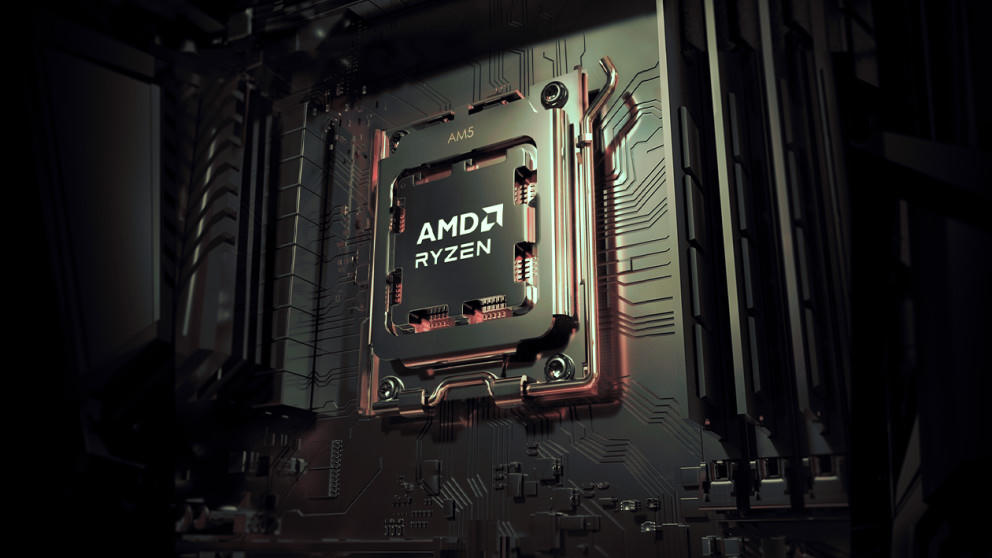
\includegraphics[height = \paperheight]{pic/cpu_hald-clut.jpg}
                    }
                    ;
                    \filldraw [white!90!fgcol]
                    (cpuMarkCenter) circle (\markMainInnerRadius)
                    ;
                    \draw [white!90!fgcol, very thick]
                    (cpuMarkCenter) circle (\markMainOuterRadius)
                    ;
                    \draw [white!90!fgcol, use path = cpuHandle, very thick] ;
                \end{scope}

                \draw (cpu.south east) ++(0, -0.3cm) coordinate (content) ;
                \node [anchor = north east]  (content) at (content) {
                    \begin{minipage} {6.0cm}
                        \raggedleft
                        \alert{CPUs} are much more capable at processing matrices that anyone of us, humans.
                        % \alert{Computers}, especially \alert{GPUs} can crunch through matrices.
                    \end{minipage}
                }
                ;
            \end{scope}

            \begin{scope} [
                    transform canvas = {
                        yshift = -0.5cm,
                        xshift = -0.5cm,
                    }
                ]
                \draw
                (current page.south) ++(1.75, 3.25) coordinate (gpuMarkCenter)
                ;
                \path [name path = gpuHandle, rounded corners = \markCornerRadius]
                (gpuMarkCenter) ++(45:\markMainOuterRadius) coordinate (gpuMarkFirst)
                (gpuMarkCenter) ++(45:(1.0cm + \markMainOuterRadius) coordinate (gpuMarkSecond)
                (gpuMarkSecond) ++(4.25, 0) coordinate (gpuMarkThird)
                (gpuMarkFirst) -- (gpuMarkSecond) -- (gpuMarkThird)
                ;
                \draw [use path = gpuHandle, very thick] ;
                \filldraw [fgcol]
                (gpuMarkThird) circle (\markSubRadius)
                ;
                \draw [fgcol]
                (gpuMarkThird) node (gpu) [right = 6pt] {
                    GPUs
                }
                ;
                \begin{scope}
                    \clip [rotate = 45, rounded corners = 0.7cm]
                    (edge) ++(0.25, -0.25) rectangle ++(10, -10)
                    ;
                    \draw
                    (edge) ++(0, -0.5) coordinate (tmp)
                    ;
                    \node [anchor = south west] (img) at (tmp) {
                        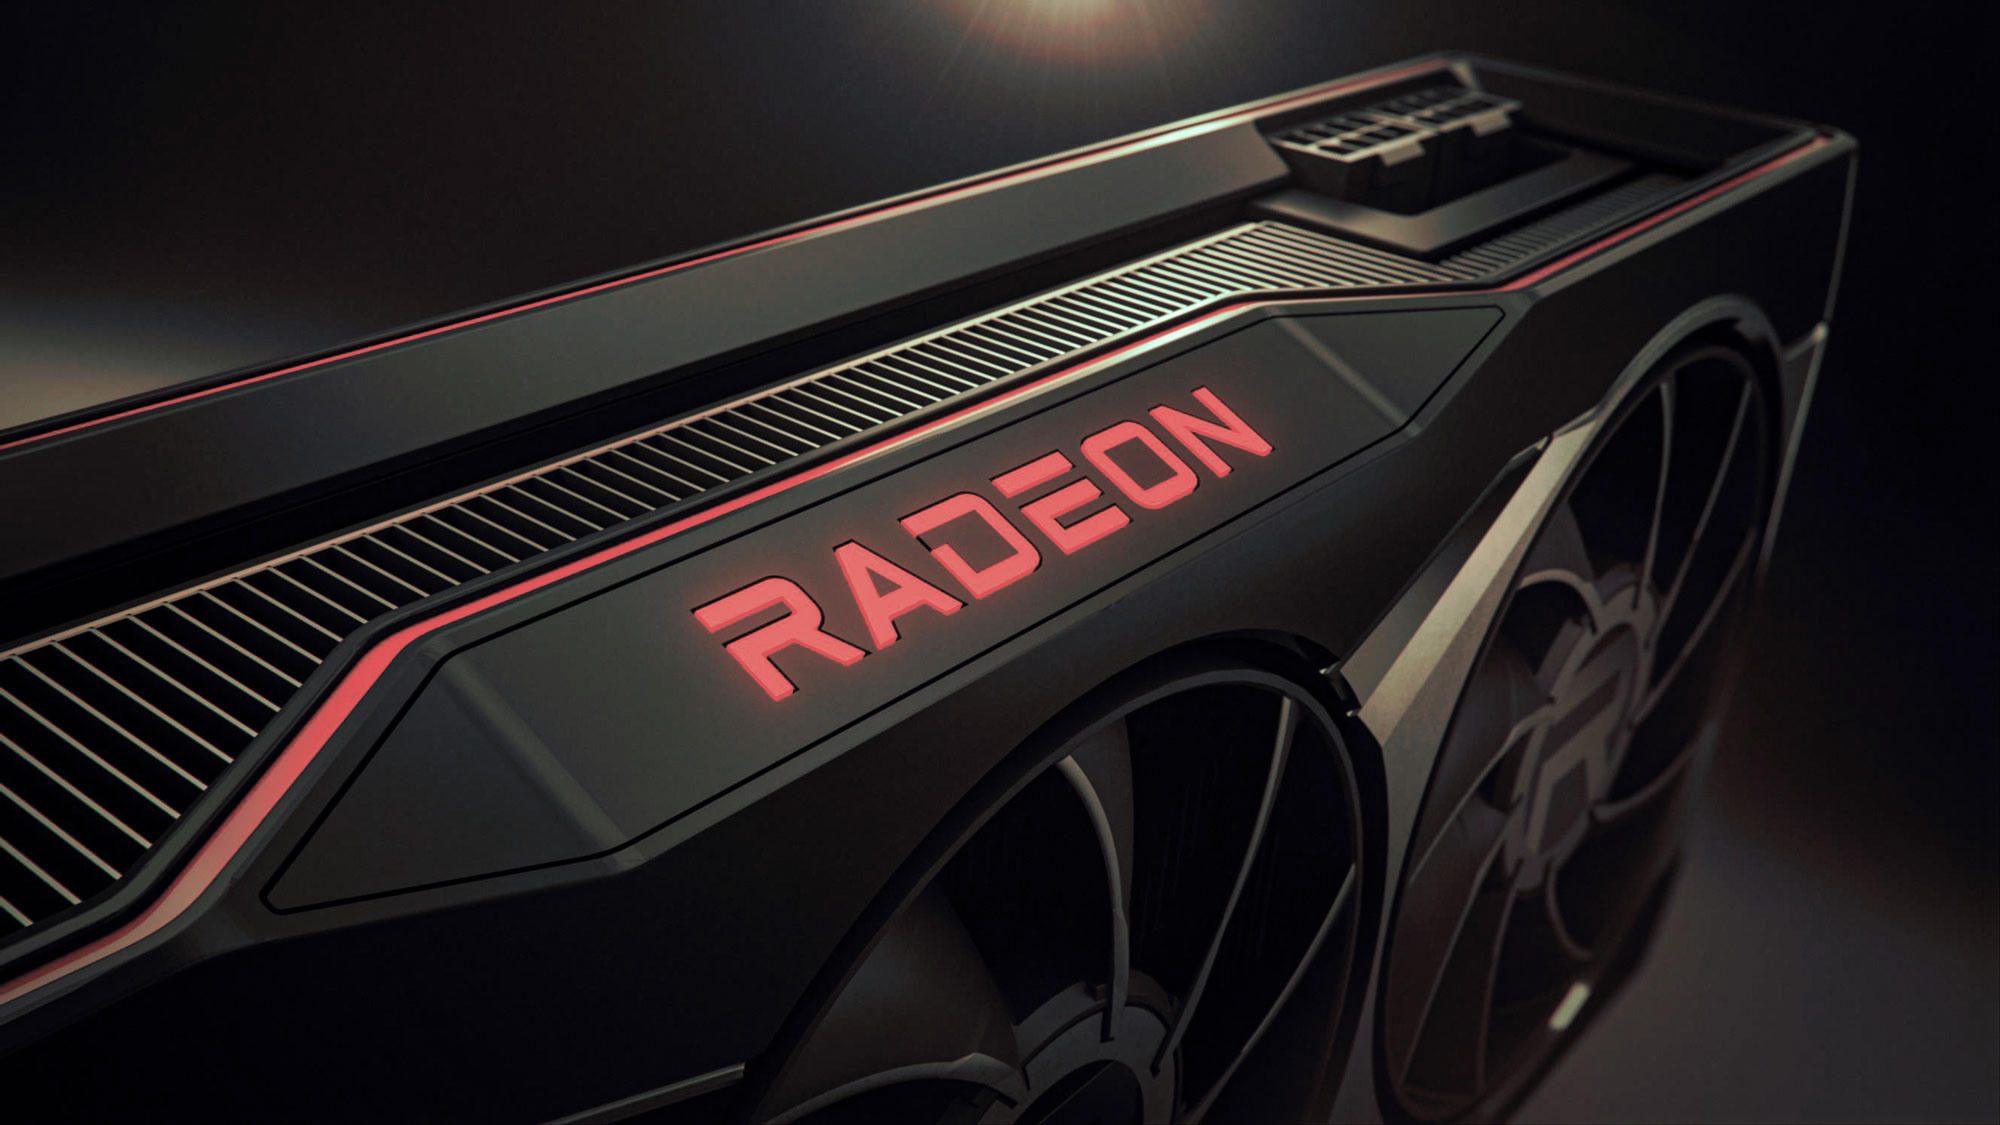
\includegraphics[height = 0.9\paperheight]{pic/gpu_hald-clut.jpg}
                    }
                    ;
                    \filldraw [white!90!fgcol]
                    (gpuMarkCenter) circle (\markMainInnerRadius)
                    ;
                    \draw [white!90!fgcol, very thick]
                    (gpuMarkCenter) circle (\markMainOuterRadius)
                    ;
                    \draw [white!90!fgcol, use path = gpuHandle, very thick] ;
                \end{scope}
                \draw (gpu.south east) ++(0, -0.3cm) coordinate (content) ;
                \node [anchor = north east]  (content) at (content) {
                    \begin{minipage} {4.0cm}
                        \raggedleft \alert{GPUs} can exploit parallelizable nature of matrix operations.
                        % \alert{Computers}, especially \alert{GPUs} can crunch through matrices.
                    \end{minipage}
                }
                ;
            \end{scope}
        \end{scope}

    \end{tikzpicture}


\end{frame}

% \begin{frame} {Weight of the Ever Growing Data}
% \end{frame}
%
% \begin{frame} {TinyML: Introduction}
% \end{frame}

\end{document}
